% two sided test for mean
% guassian with conficence region and with y axis 
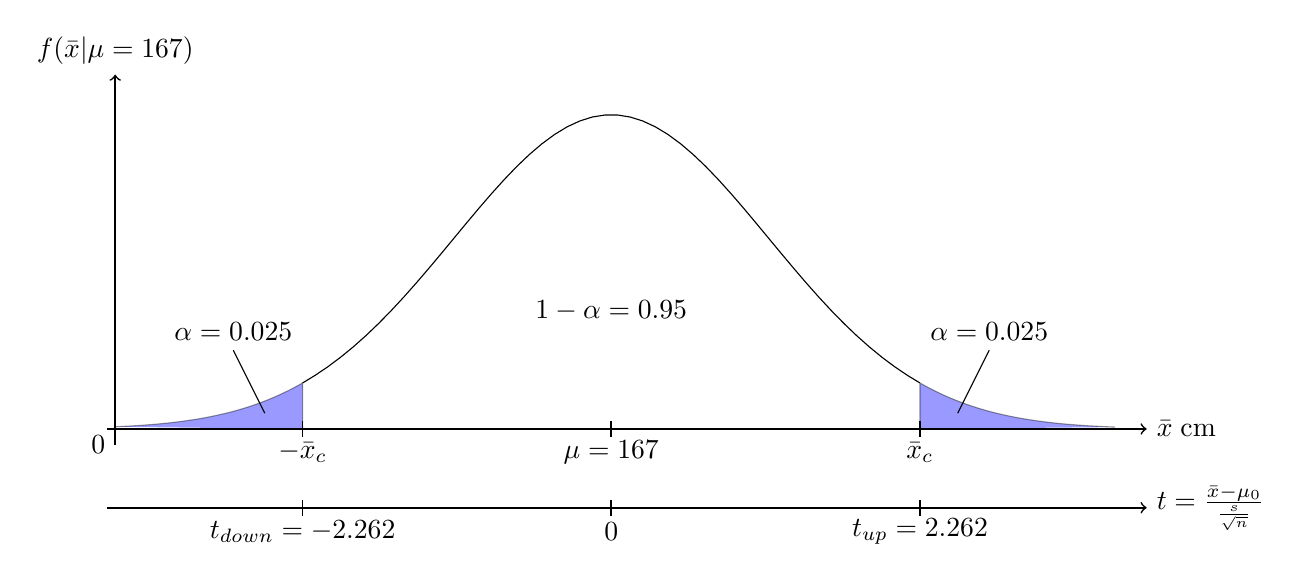
\begin{tikzpicture}[scale=2, y=5cm]
\draw[domain=-3.15:-1.96,fill=blue,opacity=0.4] (-3.15,0) plot[id=gauss1,samples=50]
(\x,{1/sqrt(2*pi)*exp(-0.5*(\x)^2)}) -- (-1.96,0);   
\draw[domain=-1.96:1.96] plot[id=gauss1, samples=50] (\x,{1/sqrt(2*pi)*exp(-0.5*(\x)^2)});   
\draw[domain=1.96:3.2,fill=blue,opacity=0.4] (1.96,0) --
plot[id=gauss3, samples=50] (\x,{1/sqrt(2*pi)*exp(-0.5*(\x)^2)});
\draw (1.96,-0.01) -- (1.96,0.01);    % ticks
\draw (-1.96,-0.01) -- (-1.96,0.01);
% ciritcal estimator values
\node at (1.96,-0.03) {$\bar{x}_c$};
\node at (-1.96,-0.03) {$-\bar{x}_c$};

% ticks on t
\draw[-,semithick] (1.96,-0.11) -- (1.96,-0.09);
\node at (1.96,-0.13)  {$t_{up}=2.262$};
\draw[-,semithick] (-1.96,-0.11) -- (-1.96,-0.09);
\node at (-1.96,-0.13)  {$t_{down}=-2.262$};
% x-axis 1
\draw[->, semithick] (-3.2,0) -- (3.4,0) node[right] {$\bar{x}$\hspace{0.1cm}cm};  
\draw[->, semithick] (-3.2,-0.1) -- (3.4,-0.1) node[right]
{$t=\frac{\bar{x}-\mu_0}{\frac{s}{\sqrt{n}}}$}; % x-axis 2
%y-axis
\draw[->, semithick] (-3.15,-0.02) node[left] {$0$} -- (-3.15,0.45)
node[above] {$f(\bar{x}|\mu=167)$}; 

\draw[-,semithick] (0,-0.01) -- (0,0.01); % zero tick on x
\draw[-,semithick] (0,-0.11) -- (0,0.-0.09); % zero tick on t
\node at (0,-0.03) {$\mu = 167$};
\node at (0,-0.13) {$0$};

% annotate alphas
\node at (0,0.15) {$1 - \alpha = 0.95$};
\draw (2.2,0.02) -- (2.4,0.1) node[above] {$\alpha = 0.025$};
\draw (-2.2,0.02) -- (-2.4,0.1) node[above] {$\alpha = 0.025$};
\end{tikzpicture} 